% a4-cayley.tex

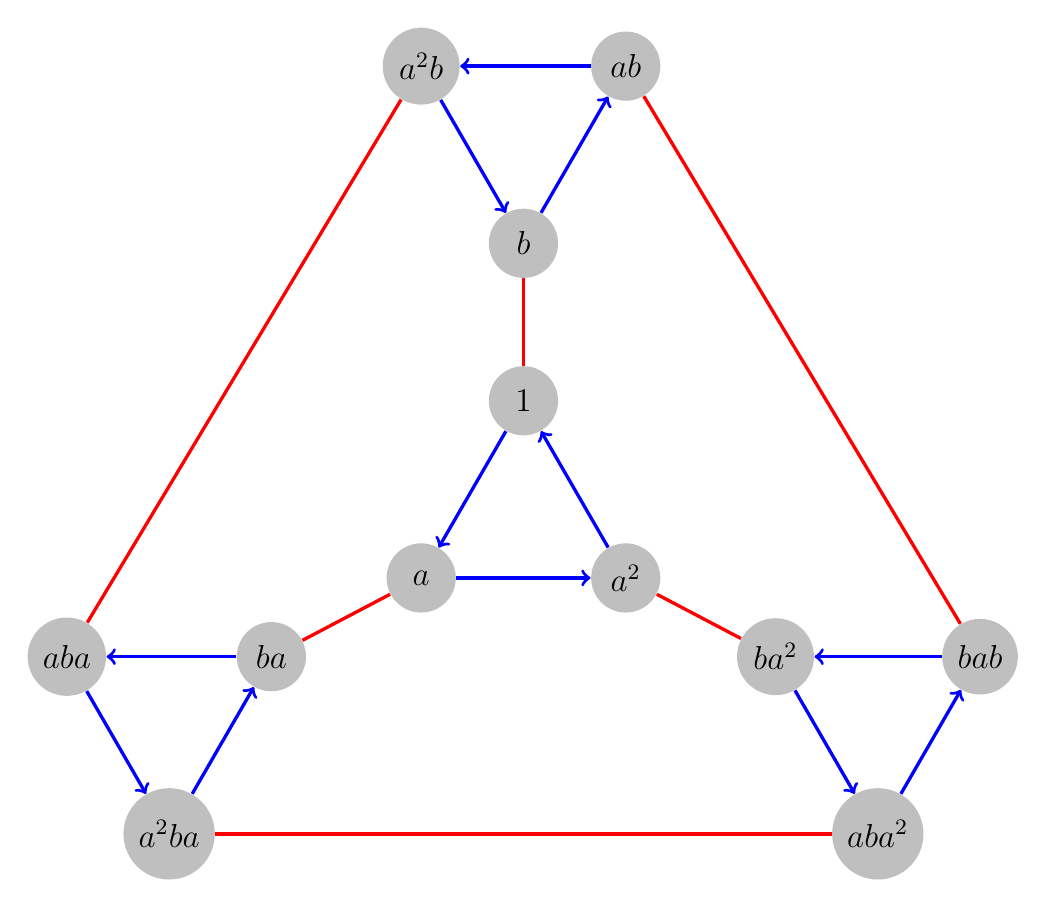
\begin{tikzpicture}[ele/.style = {circle, minimum size = 25pt, fill = lightgray, font = \large},
  a/.style = {->, blue, very thick},
  b/.style = {-, red, very thick}]
  % center 
  \foreach \angle/\label in {90/1, -30/a^2, -150/a} {
	\node (\label) [ele] at (\angle:1.5) {$\label$};
  }

  % below left
  \begin{scope}[xshift = -4.5cm, yshift = -2.5cm]
	\foreach \angle/\label in {30/ba, -90/a^2ba, -210/aba} {
	  \node (\label) [ele] at (\angle:1.5) {$\label$};
	}
  \end{scope}

  % below right
  \begin{scope}[xshift = 4.5cm, yshift = -2.5cm]
	\foreach \angle/\label in {30/bab, -90/aba^2, -210/ba^2} {
	  \node (\label) [ele] at (\angle:1.5) {$\label$};
	}
  \end{scope}

  % above
  \begin{scope}[yshift = 5.0cm]
	\foreach \angle/\label in {30/ab, -90/b, -210/a^2b} {
	  \node (\label) [ele] at (\angle:1.5) {$\label$};
	}
  \end{scope}

  \path (1) edge[a] (a)
		(a) edge[a] (a^2)
		(a^2) edge[a] (1)

		% below left
		(ba) edge[a] (aba)
		(aba) edge[a] (a^2ba)
		(a^2ba) edge[a] (ba)

		% below right
		(aba^2) edge[a] (bab)
		(bab) edge[a] (ba^2)
		(ba^2) edge[a] (aba^2)

		% above 
		(b) edge[a] (ab)
		(ab) edge[a] (a^2b)
		(a^2b) edge[a] (b)

		% b
		(1) edge[b] (b)
		(a) edge[b] (ba)
		(a^2) edge[b] (ba^2);

  \pause
  \path (a^2b) edge[b] (aba)
		(a^2ba) edge[b] (aba^2)
		(bab) edge[b] (ab);
\end{tikzpicture}
